
%(BEGIN_QUESTION)
% Copyright 2009, Tony R. Kuphaldt, released under the Creative Commons Attribution License (v 1.0)
% This means you may do almost anything with this work of mine, so long as you give me proper credit

In this process, maple syrup is heated as it passes through a steam heat exchanger, then enters an evaporator where the water boils off.  The purpose of this is to raise the sugar concentration of the syrup, making it suitable for use as a food topping.  A level control system (LT, LIC, and LV) maintains constant syrup level inside the evaporator, while an analytical control system (AT, AIR, AC, and AV) monitors the sugar concentration of the syrup and adjusts steam flow to the heat exchanger accordingly.

$$\includegraphics[width=15.5cm]{i02936x01.eps}$$

Suppose the syrup analyzer (AT) suffers a sudden calibration problem, causing it to register too low (telling the analytical controller that the sugar concentration of the syrup is less than it actually is).

\vskip 10pt

Describe in detail the effect this calibration error will have on the performance of the analytical control system.

\vskip 20pt \vbox{\hrule \hbox{\strut \vrule{} {\bf Suggestions for Socratic discussion} \vrule} \hrule}

\begin{itemize}
\item{} What economic effect will this mis-calibration have on the process?  In other words, does the process become more or less profitable as a result of this change?
\item{} Suppose someone shuts the manual block valve on the steam line just a little bit, so that it is about 80\% open instead of 100\% open.  How will this process change affect the control systems in this process?
\end{itemize}

\underbar{file i02936}
%(END_QUESTION)





%(BEGIN_ANSWER)

The syrup's sugar concentration will eventually become {\it excessive} as the analytical controller (AC) attempts to maintain setpoint.

%(END_ANSWER)





%(BEGIN_NOTES)

\vskip 20pt \vbox{\hrule \hbox{\strut \vrule{} {\bf Virtual Troubleshooting} \vrule} \hrule}

This question is a good candidate for a ``Virtual Troubleshooting'' exercise.  Presenting the diagram to students, you first imagine in your own mind a particular fault in the system.  Then, you present one or more symptoms of that fault (something noticeable by an operator or other user of the system).  Students then propose various diagnostic tests to perform on this system to identify the nature and location of the fault, as though they were technicians trying to troubleshoot the problem.  Your job is to tell them what the result(s) would be for each of the proposed diagnostic tests, documenting those results where all the students can see.

During and after the exercise, it is good to ask students follow-up questions such as:

\begin{itemize}
\item{} What does the result of the last diagnostic test tell you about the fault?
\item{} Suppose the results of the last diagnostic test were different.  What then would that result tell you about the fault?
\item{} Is the last diagnostic test the best one we could do?
\item{} What would be the ideal order of tests, to diagnose the problem in as few steps as possible?
\end{itemize}



%INDEX% Basics, control loop troubleshooting: determining effect of specified fault(s)
%INDEX% Process: maple syrup concentration (single-effect evaporator)

%(END_NOTES)


